\section{Theoretische Grundlagen}
\label{sec:theorie}

Im Folgenden werden zunächst einige theoretische Grundlagen von Ionenkristallen näher beleuchtet.

\subsection{Dotierung von Ionenkristallen}

Ordnen sich die Ionen eines Salzes in einer Gitterstruktur an, spricht man von Ionenkristallen. 
Dabei ordnen sich ein Kation und ein Anion immer so an, dass sich mikroskopische Dipole ausbilden, makroskopisch gesehen aber ein vollständig neutraler Kristall entsteht. \\
In der Theorie entsteht eine perfekte Kristallstruktur, doch in der Realität kommt es, wie in \autoref{fig:punktdefekte} dargestellt, zu Punktdefekten.
So können Gitterplätze unbesetzt sein, sodass eine Leerstelle entsteht, oder auch überbesetzt sein, sodass eine Zwischenstelle, die theoretisch unbesetzt sein sollte, dennoch besetzt ist.

\begin{figure}[H]
    \centering
    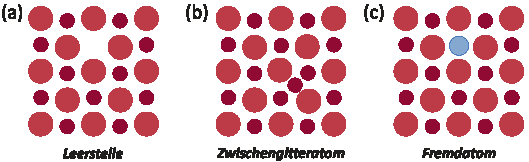
\includegraphics[]{figures/Fehlstellen.pdf}
    \caption{Beispiele für in (Ionen-)Kristallen auftretende Punktdefekte: (a) Leerstelle, (b) Zwischengitteratom, (c) Fremdatom \cite[S. ~38]{grossmarx}}
    \label{fig:punktdefekte}
\end{figure}

Für den Prozess der Dotierung, bei der durch die Einführung von Fremdionen in das Gitter größere Dipole erzeugt werden, sind vor allem die Leerstellen interessant.
Da die so eingeführten Ionen aber nicht zwangsläufig dieselbe Ladung wie die des ursprünglichen Gitters besitzen, muss die entstehende Ladungsdiskrepanz vom Gitter kompensiert werden.
Ionen in der Nähe wandern so je nach Ladung Richtung Oberfläche, oder sammeln sich um das eingeführte Fremdion. \\
Mikroskopisch herrscht weiterhin Ladungsneutralität, von außen gesehen wird der Ionenkristall durch die Dotierung aber leicht geladen.

\subsection{Dipolrelaxation}

Die so entstehenden Dipole zeigen in Anwesenheit eines elektrischen Feldes ein charakteristisches Verhalten.
Mit der potentiellen Energie
\begin{equation}
    E_\text{pot} = - \vec{p} \cdot \vec{E} \,,
    \label{eq:potE}
\end{equation}
wobei $\vec{p}$ das Dipolmoment und $\vec{E}$ das elektrische Feld darstellen, ist offensichtlich, dass der energetisch günstigste Zustand genau dann angenommen wird, 
wenn sich die durch die Dotierung eingeführten Dipolmomente parallel zum Feld ausrichten. \\

Ohne äußeres Feld richten sich die Dipolmomente ohne Präferenz in eine zufällige Raumrichtung aus, sodass sich ein Gesamtdipolmoment von null ergibt. \\
In einem homogenen elektrischen Feld (bei Raumtemperatur) minimiert sich also die potentielle Energie genau dann, wenn die Dipole genug Energie erhalten, um die Aktivierungsenergie $W$, 
die zur Überwindung der Coulomb-Barriere im Gitter nötig ist, erhalten und sich so entlang des Feldes ausrichten können.
Kann diese Aktivierungsenergie nicht aufgebracht werden, sitzen die Leerstellen und Dotier-Ionen, eingeschränkt vom Gitterpotential, örtlich fest. \\
Zur Beschreibung des Relaxationsprozesses nach Ausschalten des E-Feldes, also der Rückkehr in den zufällig ausgerichteten Zustand der Dipolmomente, erfolgt durch die Maxwell-Boltzmann-Verteilung nach
\begin{equation}
    \tau(T) = \tau_0 \text{e}^{\frac{W}{k_\text{B} T}}  \,,
\end{equation}
mit der Boltzmannkonstante $k_\text{B}$, Temperatur $T$ und $\tau_0 = \tau(\infty)$ \cite{v48}.





